%----------------------------------------------------------------------------------------
%   Final Year Project Report Bachelor of Engineering
%   Glasgow College, UESTC
%   (LaTex Template)
%-------------------------------------------------------------------------------
% Arrangement Author:   Huang Yifan  2288862h@student.gla.ac.uk
%                       Zhuheng Song 2357651S@student.gla.ac.uk
%-------------------------------------------------------------------------------
%    PACKAGES AND OTHER DOCUMENT CONFIGURATIONS
%-------------------------------------------------------------------------------

% arrangement ------------------------------------------------------------------
\documentclass[
    12pt, % The default document font size, options: 10pt, 11pt, 12pt
    twoside, % Two side (alternating margins) for binding
    % draft,  % speed up comile and show problems
    % showframe, % Uncomment to show how the type block is set on the page
]{article} % The class file specifying the document structure

\usepackage[
    a4paper,
    inner=2.5cm,  % more margin for inner in case to bookbind
    outer=2cm,
    top=2cm,
    bottom=2cm
]{geometry}

% set line spacing to 1.5
\usepackage{setspace}
\onehalfspacing{}
% set no vertical space to lists
\usepackage{enumitem}
\setlist{itemsep=0mm}

% language, fonts and symbols --------------------------------------------------
% \usepackage{xeCJK}  % chinese character support
% \usepackage{fontspec}
% \setromanfont{Times New Roman}
% \setsansfont{Arial}
% \setmonofont{Courier New}
\usepackage{csquotes}  % quotation support
\usepackage{amssymb}  % math symbols support

% figures, tables, code --------------------------------------------------------
\usepackage[figuresleft]{rotating}  % for figure rotation
\usepackage{graphicx}  % inclusion of graphics files
\graphicspath{{./}}
\usepackage{import}  % to solve import path
\usepackage[newfloat]{minted}
\SetupFloatingEnvironment{listing}{name=Program code}
\SetupFloatingEnvironment{listing}{listname=List of Program Code}
\usemintedstyle{vs}
\usepackage{caption}

\usepackage{tabularx}
\usepackage{booktabs}  % for \toprule, \midrule, \bottomrule

\usepackage[nottoc]{tocbibind}  % add LofF, LofT to TOC

% reference --------------------------------------------------------------------
\usepackage[
    backend=biber,
    style=alphabetic,
    citestyle=authoryear,
    backref=true,
    maxcitenames=1,
    maxbibnames=999,
    sorting=ynt,
]{biblatex}
% set cite link to whole author-year
\makeatletter
    \let\abx@macro@citeOrig\abx@macro@cite{}
    \renewbibmacro{cite}{\bibhyperref{\let\bibhyperref\relax\relax\abx@macro@citeOrig{}}}
\makeatother{}
% allow \citetitle{} to support hyperlink
\DeclareCiteCommand{\citetitle}{\usebibmacro{prenote}}{
    \ifciteindex{\indexfield{indextitle}}{}\printtext[bibhyperref]{\printfield[citetitle]{labeltitle}}
}{\multicitedelim}{\usebibmacro{postnote}}
% add bibliography files
\addbibresource{References.bib}

% color ------------------------------------------------------------------------
\usepackage[svgnames]{xcolor}  % colouring
\definecolor{blue_cite}{RGB}{34,111,212}

\usepackage{hyperref}  % keep hyperref to be loaded last (before glossaries-extra)
\hypersetup{
    colorlinks=true,
    linkcolor=DarkSalmon,
    % anchorcolor=black,
    citecolor=blue_cite,
    % filecolor=cyan,
    % menucolor=red,
    % runcolor=cyan,
    urlcolor=cyan,
    % allcolors=LightSlateGray,
}  % set colors for different types of links

% list of symbols --------------------------------------------------------------
\usepackage[symbols, nogroupskip, record]{glossaries-extra}  % place after hyperref
\GlsXtrLoadResources[
 src={Notations.bib},
 type=symbols,
 save-locations=false
]
%----------------------------------------------------------------------------------------
%    THESIS INFORMATION (NECESSARY)
%----------------------------------------------------------------------------------------
\newcommand{\thesistitle}{Some Thesis Title}  % Your thesis title, this is used in the cover page, print it elsewhere with \thesistitle
\newcommand{\GUID}{1111111A}  % Your GUID, this is used in the cover page, print it elsewhere with \GUID
\newcommand{\student}{San~\textsc{Zhang}}  % Your name, this is used in the title page and abstract, print it elsewhere with \student
\newcommand{\firstsupervisor}{\textcolor{red}{\tiny Keep blank before hardcopy submission}}  % Your 1st supervisor's name, this is used in the cover page, print it elsewhere with \firstsupervisor. YOU NEED TO KEEP BLANK FOR MOODLE SUBMISSION BUT PUT THE NAME BEFORE HARDCOPY SUBMISSION.
\newcommand{\secondsupervisor} {\textcolor{red}{\tiny Keep blank before hardcopy submission}}  % Your 2nd supervisor's name, this is used in the cover page, print it elsewhere with \secondsupervisor. YOU NEED TO KEEP BLANK FOR MOODLE SUBMISSION BUT PUT THE NAME BEFORE HARDCOPY SUBMISSION.
%----------------------------------------------------------------------------------------
%    OTHER INFORMATION
%----------------------------------------------------------------------------------------
\newcommand{\degree}{Engineering}  % Your degree name, this is used in the cover page and abstract, print it elsewhere with \degree
\newcommand{\subject}{Electric & Electronic Engineering}  % Your subject area, this is not currently used anywhere in the template, print it elsewhere with \subject
\newcommand{\keywords}{}  % Keywords for your thesis, this is not currently used anywhere in the template, print it elsewhere with \keywords
\newcommand{\university}{\href{https://www.uestc.edu.cn/}{UETSC}}  % Your university's name and URL, this is used in the cover page and abstract, print it elsewhere with \university
\newcommand{\department}{\href{http://www.gla.uestc.edu.cn/}{Glasgow College}}  % Your department's name and URL, this is used in the cover page and abstract, print it elsewhere with \department
%----------------------------------------------------------------------------------------
%    ENVIRONMENTS
%----------------------------------------------------------------------------------------
\newenvironment{declaration}{
    \newgeometry{left=2cm, right=2cm, top=2cm, bottom=2cm}
    \renewcommand*{\arraystretch}{1.3}
    \section*{Coursework Declaration and Feedback Form}
    % \addcontentsline{toc}{section}{Coursework Declaration and Feedback Form}
}{\clearpage\restoregeometry}

\renewenvironment{abstract}{
    \section*{Abstract}
    \bigskip
    \addcontentsline{toc}{section}{Abstract}
}{\clearpage}

\newenvironment{acknowledgement}{
    \section*{Acknowledgements}
    \bigskip
    \addcontentsline{toc}{section}{Acknowledgements}
}{\clearpage}

\newenvironment{code}{
    \captionsetup{type=listing}
}{}

\AtBeginDocument{
    \hypersetup{pdftitle=\thesistitle} % Set the PDF's title to your title
    \hypersetup{pdfauthor=\student} % Set the PDF's author to your name
    \hypersetup{pdfkeywords=\keywords} % Set the PDF's keywords to your keywords
}

\begin{document}
%----------------------------------------------------------------------------------------
%    COVER PAGE
%----------------------------------------------------------------------------------------
\begin{titlepage}
    \begin{center}
        
\includegraphics{Figures/Badge.jpg}
        \vspace*{.08\textheight}

        \textsc{\Large Final Year Project Report\\Bachelor of Engineering}\\[2cm] % Thesis type

        {\LARGE \bfseries \thesistitle\par}\vspace{3cm}% Thesis title

        \begin{minipage}[t]{0.4\textwidth}
            \begin{flushleft} \LARGE
                Student:\\
                \vspace*{.02\textheight}
                GUID:\\
                \vspace*{.02\textheight}
                \(1^{st}\) Supervisor:\\
                \vspace*{.02\textheight}
                \(2^{nd}\) Supervisor:\\
            \end{flushleft}
        \end{minipage}
        \begin{minipage}[t]{0.4\textwidth}
            \begin{flushright} \LARGE
                \student{}\\
                \vspace*{.02\textheight}
                \GUID{}\\
                \vspace*{.02\textheight}
                \firstsupervisor{}\\
                \vspace*{.02\textheight}
                \secondsupervisor{}\\
            \end{flushright}
        \end{minipage}\\[1.5cm]

        \vfill
        {\huge 2020--2021}\\[3cm]
    \end{center}
\end{titlepage}
%----------------------------------------------------------------------------------------
%    DECLARATION PAGE
%----------------------------------------------------------------------------------------
\begin{declaration}
    \pagestyle{empty}  % empty header, no page number footer
    % set separation of above and below the rules to 0
    \renewcommand{\aboverulesep}{0pt}
    \renewcommand{\belowrulesep}{0pt}
    \setlength\heavyrulewidth{0.4pt}
    \setlength\lightrulewidth{0.4pt}

    \textit{This Student should complete and sign this part}
    \begin{table}[!ht]
        \large
        \begin{tabularx}{\textwidth}{|X|X|}
            \toprule
            Student Name:                           & Student GUID:                                                                                    \\
            \student{}                              & \GUID{}                                                                                          \\
            \midrule
            Course Code:                            & Course Name:                                                                                     \\
            UESTC4006P                              & INDIVIDUAL PROJECT 4                                                                             \\
            \midrule
            Name of 1st Supervisor:                 & Name of 2nd Supervisor:                                                                          \\
            \firstsupervisor{}                      & \secondsupervisor{}                                                                              \\
            \midrule
            \multicolumn{2}{|l|}{Title of Project:}                                                                                                    \\
            \multicolumn{2}{|p{15cm}|}{{\Large\thesistitle}}                                                                                  \\
            \midrule
            \multicolumn{2}{|l|}{\textbf{Declaration of Originality and Submission Information}}                                                       \\
            \midrule
            \small{I affirm that this submission is all my own work in accordance with the University of Glasgow Regulations and the School of Engineering requirements}
                                                    & {}                                                                                               \\
            \small{Signed (Student):}               & {}                                                                                               \\
            \raggedright{\small{I affirm that this submission is completed by the student independently and the quality of the submission meets the requirements for graduation. I consent to the student taking part in the oral presentation.}}
                                                    & \multicolumn{1}{|c|}{\raisebox{-\totalheight}{\centering
\includegraphics[scale=0.7]{Figures/BarCode.jpg}}} \\
            \small{Signed (\(1^{st}\) Supervisor):} & {}                                                                                               \\
            \midrule
            \multicolumn{2}{|l|}{Date of Submission:}                                                                                                  \\
            \midrule
            \multicolumn{2}{|l|}{\textit{\normalsize{Feedback from Lecturer to Student to be completed by Lecturer or Demonstrator}}}                               \\
            \midrule
            \multicolumn{2}{|l|}{Grade Awarded:}                                                                                                       \\
            \multicolumn{2}{|l|}{Feedback (as appropriate to the coursework which was assessed):}                                                      \\
            \multicolumn{2}{|l|}{}                                                                                                                     \\
            \multicolumn{2}{|l|}{}                                                                                                                     \\
            \midrule
            Lecturer Demonstrator:                  & Date returned to the Teaching Office:                                                            \\
            {}                                      & {}                                                                                               \\
            \bottomrule
        \end{tabularx}
    \end{table}
\end{declaration}

%----------------------------------------------------------------------------------------
%    ABSTRACT PAGE
%----------------------------------------------------------------------------------------
\pagenumbering{roman}  % start to show page number in the roman style

\begin{abstract}

All reports start with an abstract, which contains a summary of the project: its
aim, what was done and, most important, what was achieved. This document
describes the requirements for a project report in the School of Engineering and
gives advice on how to get better marks. It is structured to match a project
report as far as possible so that the document can be used as a template.

\end{abstract}

%----------------------------------------------------------------------------------------
%    ACKNOWLEDGEMENTS
%----------------------------------------------------------------------------------------
\begin{acknowledgement}
    The acknowledgments and the people to thank go here, don't forget to include
    your project advisor
\end{acknowledgement}

%----------------------------------------------------------------------------------------
%    LIST OF CONTENTS
%----------------------------------------------------------------------------------------
\tableofcontents
\pagebreak
%----------------------------------------------------------------------------------------
%    LIST OF FIGURES AND TABLES
%----------------------------------------------------------------------------------------
\listoffigures
\listoftables
\listoflistings
\pagebreak
%----------------------------------------------------------------------------------------
%    LIST OF NOTATIONS
%----------------------------------------------------------------------------------------
\printunsrtglossary[type=symbols,style=long,title={List of Notations}]
\pagebreak
%----------------------------------------------------------------------------------------
%    THESIS CONTENT - SECTIONS
%----------------------------------------------------------------------------------------
\pagestyle{headings} % Return the page headers back to the "thesis" style
\pagenumbering{arabic}

% Include the sections of the thesis
\section{Introduction}

Whew – I’ve finished the work, now I only have to write the report. Sound
familiar? Many students put off writing until too late and don’t leave enough
time to make a good job of the report. This is a serious mistake because the
report typically accounts for a large fraction of the assessment. Start early
because most people find report-writing difficult. Think about the report
throughout your project, keep track of references and collect material to
illustrate the report.

\textbf{The report contributes a large fraction of the overall assessment for
    the project.} It is depressingly common for students to perform excellent
technical work but submit a weak report, which pulls their overall result down.
Please apportion your time appropriately.

\subsection{What are the important parts of a report?}

It’s worth thinking of the sort of report that you might submit to your managers
in your future career. The technical content of the report can be broken into
two parts.

\begin{itemize}
    \item a description of the work that you did and the results that you
          obtained
    \item your analysis of the results and what you learned from them – the
          conclusions.
\end{itemize}

It is likely that your managers will open the report at the conclusions and
perhaps look back at the analysis if they want to see the evidence for a
particular point. It is most unlikely that they will read the earlier sections
at all. The report that you are writing now is an academic document and we will
read it all but the same point applies: the analysis and conclusions are the
most important sections. These are where you can show your understanding and
insight and they therefore make a major impact on your final grade. Make sure
that you spend enough time on them.

\subsection{Mechanical aspects}

The length of the body of the report is specified in the instructions for the
project. Extra material may be provided in appendices but this material is for
reference only: you cannot assume that the reader will study it. In other words,
do not put vital points in an appendix.

You probably think that the report is too short but this is deliberate. Most
reports are submitted to busy managers, who do not have time to read lengthy
documents. It is important to learn how to pick out the vital points and write a
concise report with maximum impact.

Reports should be word-processed and firmly bound. Use A4 paper and a clear
typeface such as 12-point Times\footnote{Cambria is better if you use a lot of
    mathematics in Word because it is used automatically for equations.}, number the
pages and leave margins of at least 25 mm all round. Follow the layout of this
document.

\begin{itemize}
    \item The front cover shows the title of the project with your name(s) and
          matriculation number(s).
    \item The abstract goes on the next page. It should be about 100–250 words
          and gives a brief summary of the report including the background and
          aims of the project, the principal results and conclusions.
    \item You may wish to include a page with acknowledgements next.
    \item The following page has the table of contents. There is no need for
          lists of figures and tables.
    \item The body of the report should be divided into numbered sections, each
          starting on a new page. Figures (diagrams, plots or photographs) and
          tables need captions and should be numbered.
    \item References follow the body of the report, again starting on a new
          page.
    \item Any appendices should again start on new pages. Number them
          alphabetically (Appendix A and so on).
\end{itemize}

\subsection{What goes into the introduction?}

Explain the background to the project and the reasons why your particular piece
of work was considered worthwhile. This usually includes a literature review to
show how your project builds on established knowledge. A worthwhile review must
be critical, meaning that you assess the previous publications to show where
more work is needed. A simple summary of previous work is of little value
because the reader can get this by scanning the references. Do not quote from
advertising material and do not make the literature review too long, definitely
less than 25\% of the report.

The introduction leads to the aims of the project: what you are trying to
achieve. Be specific.
\section{Body of the report}

This section describes the structure of different types of report and how the
text should be written. It includes tips for diagrams and equations, which are
required for most engineering reports. Finally, it addresses the vital topic of
references and how you should acknowledge the work of others.

\subsection{Structure and sections}

The structure of the report and the titles of sections depend on the nature of
the project. Here are suggestions for two extreme types, which can be adjusted
to suit your report.

\subsubsection{Research projects}

Here you are given a starting point and a general direction: your aim is to
discover something new. The report would probably be divided into sections with
familiar titles.

\begin{itemize}
    \item \textbf{Theory} {--} Explain essential background theory that is vital
          for the reader to understand your report. Select and present the
          material to show its relevance to the project and demonstrate your
          understanding. Do not repeat standard material from textbooks, which
          is a waste of space; give a reference instead. This section should
          lead into the Objectives of your project: the specific questions that
          your research will address.
    \item \textbf{Experimental Techniques} {--} Give an account of your
          experimental or numerical techniques. Emphasise details that would be
          necessary to continue the work or to compare your results with those
          of other experimenters. Include what you would have liked to know at
          the start of your project but don’t copy material from manuals or
          other references.
    \item \textbf{Results} {--} Describe these at an appropriate level of detail to
          support your conclusions. Be selective: you cannot include everything.
          Lengthy tables should be left to an appendix. Avoid unnecessary
          detail: describe preliminary experiments briefly if at all, unless
          they illustrate some important point.
\end{itemize}

\subsubsection{Design, build and test projects}

Here the goal is specified, more or less precisely: your job is to work out how
to get there. The titles of the sections are less standardised but here is a
possible approach.

\begin{itemize}
    \item \textbf{Specification} {--} Typically you are given only a vague
          description of the functions required as the aims and must first
          develop this into a firm specification against which your final
          product will be judged. This may be a fairly long section because you
          need to justify your choices. The detailed specification provides the
          objectives for this type of project.
    \item \textbf{Possible strategies} {--} Evaluate briefly the possible
          approaches that you considered and explain why you selected one of
          these. Avoid excessive detail of discarded possibilities.
    \item \textbf{Implementation} {--} Describe the final product. Concentrate
          on key features that required advanced design and skim over well-known
          aspects. Mention useful points that might help future students, such
          as tricky sections of data sheets.
    \item \textbf{Testing} {--} This is equivalent to the ‘Results’ section of a
          research project.
\end{itemize}

\subsection{Style of writing}

One of the most difficult aspects of writing is to judge the level and
background of your readers. Typically the report is assessed by your first
supervisor, who is an expert on the topic, and your second supervisor, who is
not. You should therefore assume that the reader is a \textit{well-educated,
    graduate engineer} but not an expert on the subject of the project. Assume that
he or she is familiar with the general concepts taught in courses up to level 3
but not with the details of specialised courses at higher levels.

It is also difficult to appreciate that most readers are not interested in the
nitty-gritty detail. They want to know \textit{what} you did and \textit{why}
you did it that way but they don’t want a step-by-step account of \textit{how}
you did it. Your watchword should therefore be:

\begin{center}
    \large\textbf{SUMMARISE!}
\end{center}

Of course some people need the details {--} a person continuing work on the
project requires precise experimental methods, for instance. Such material is
best in an appendix. The same is true for computer programs and schematics of
complicated circuits. Design-and-build projects may need a User’s Manual, which
should be included as an appendix.

A report is a formal document and should be written in appropriate language.
Numerous books offer advice on writing reports and a selection [1, 2, 3, 4] is
listed in the references at the end. Here are a few tips.

\begin{itemize}
    \item Reports should be written in correct English. Break text into
          paragraphs, keep sentences to a reasonable length and insert
          appropriate punctuation. Use a spell-checker and a grammar-checker if
          desired but neither is a substitute for careful reading.
    \item A report is not a story. Write ‘The voltage was measured’ rather than
          ‘I measured the voltage’. This document contains instructions and
          therefore uses a different style.
    \item Define all abbreviations when they are first used: ‘The accelerometer
          uses a serial peripheral interface (\gls{spi})’. Provide a list of
          abbreviations if you use a large number of them.
    \item Don’t write material that you don’t understand. It will be obvious to
          the reader.
\end{itemize}

\subsection{Precision}

An engineering report must be precise. This applies both to the language and to
numerical values. For example, the words precision and accuracy are often used
interchangeably in non-technical discussion but the distinction between them is
vital in engineering. Vague, waffly text is a major weakness of many students’
technical reports (and examination answers).

Quote numerical results to an appropriate number of significant figures. For
example, it is pointless to claim that a length was 12.345 mm if it was measured
with a pocket ruler. Don’t simply write down all the digits displayed on your
calculator.

Analyse the uncertainties in your results to increase the impact of your
results. Please avoid horrors like this:

\begin{displayquote}
    The gain was quite accurate.
\end{displayquote}

The sentence is meaningless and the reader will doubt whether you have any idea
of the accuracy. Contrast this sentence:

\begin{displayquote}
    The accuracy of the gain was estimated to be \(\pm2\%\), limited by the
    tolerance of the resistors. A detailed analysis is given in Appendix C.
\end{displayquote}

This is informative and convinces the reader that you have a full understanding.

\begin{figure}[htb]
    \centering{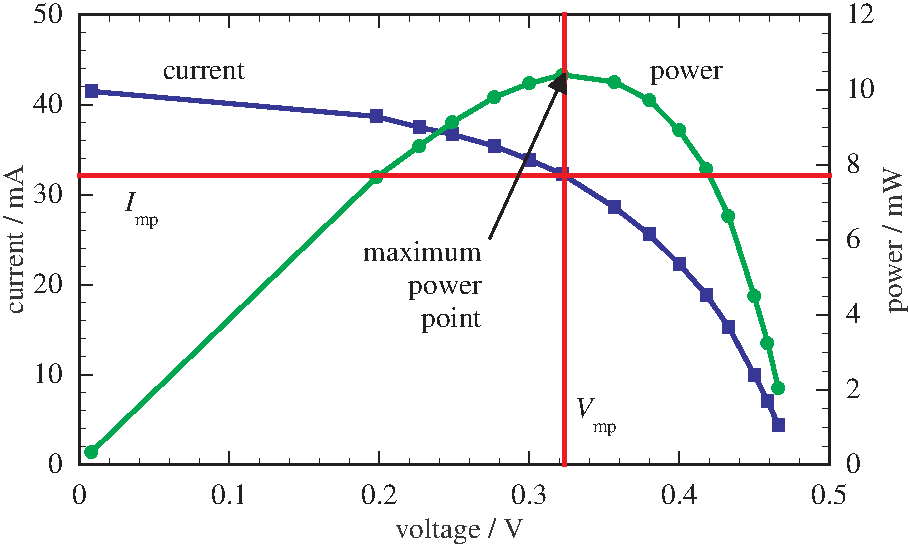
\includegraphics[width=0.7\textwidth]{Figures/solarcell.pdf}}
    \caption[Current and Power as A Function of Voltage Delivered by A Single
        Photovoltaic Cell]{Current and power as a function of voltage delivered by a
        single photovoltaic cell: under illumination from a 150 W metal halide
        floodlamp, showing the maximum power point.}\label{f:solarcell}
\end{figure}

\subsection{Figures and tables}

Figures (diagrams, photographs etc) and tables must have informative captions
and be numbered as in \autoref{f:solarcell}. Axes of graphs should have scales,
titles and units, otherwise the plot is meaningless. Multiple curves must be
labelled, either directly as in \autoref{f:solarcell} or with a caption. Use
dotted or dashed lines as well as colour for clarity; remember that the reader
might be colour-blind or have only a black-and-white printout. All text must be
legible, roughly the same size as the main text. Be warned that plots from Excel
or Matlab need extensive editing to bring them up to an acceptable standard.
Experimental traces can be captured on most modern test equipment and can make
good illustrations.

Never use screenshots or images taken with a camera where a more professional
method is available.

Be careful if you paste figures into Microsoft products, which seem to wreck
almost any format; png files may be best. Do not distort the image by changing
the aspect ratio (width:height).

Tables must have appropriate headings with units. Avoid lengthy tables: consider
whether a graph would be clearer or the data would be better in an appendix.

\subsection{Equations}

Most engineering reports contain equations. Do not type these as though they are
ordinary text in Word but use an equation editor. Short equations, such as
\(ax^2+bx+c=0\), can be written inline but longer equations should be displayed
like this:

\begin{equation}
    x=\frac{-b\pm\sqrt{b^2-4ac}}{2a}
\end{equation}

Number equations so that you can refer to them. Consider \LaTeX{} if you have a
lot of mathematics.

\subsection{Software}

It is tricky to describe software well. Often the best approach is to describe
the high-level structure in the main text (a UML diagram for example) and pick
out any special features of the program that need to be explained in detail. A
complete listing should be included as an appendix. Do not describe your
complete code line by line; you will send the reader to sleep. Please make sure
that the listing is formatted to make it easy to read and understand;
screenshots are unacceptable.

You must supply references to make it clear where your computer code includes
material from elsewhere, such as published libraries or code examples. This is a
perfectly acceptable approach (it is why the material is made available) but you
must:

\begin{itemize}
    \item provide a reference to the source of the material
    \item use comments in the listings to make it absolutely clear which parts
          were written by you and which were taken from published material.
\end{itemize}

If you do not do this, the reader will assume that the code is all your own work
and you will be guilty of plagiarism if this is not correct. See the next
section.

\subsection{References}

No project is done in isolation. A research project builds on the results of
previous workers; a design-and-build project depends on the properties of the
components available. You therefore draw on published documents during your
project and must provide references to these sources in your report. References
are cited (a) to give due credit to the originator and (b) to guide a reader who
wants more detailed information. You should give a reference wherever it is
required for either of these purposes. Properly referenced material from many
sources is a sign of a good project report.

References must be cited with sequential numbers in square brackets where they
are used in the text. Typical usage is `Fitzmaurice and Hand
\autocite{fitzmaurice1987comparison} showed that\ldots’ or `The median is an
appropriate estimator for this signal \autocite{fitzmaurice1987comparison}'

Avoid direct quotations from references in general; make it absolutely clear
that the text is a quotation if this is unavoidable. An illustration, such as a
diagram from a data sheet, is another type of quotation and must be referenced,
typically in the figure caption. This is perfectly acceptable: do not waste time
redrawing diagrams.

\subsubsection{Plagiarism}

If you copy from another person’s work (project report, book, journal, code, web
page or any other document) without acknowledging the source, you are guilty of
plagiarism. This is a disciplinary offence and the University has procedures for
handling it. The failure to acknowledge a source is considered as plagiarism
even if there was no deliberate intention to cheat.

Avoid any risk of plagiarism by providing a reference for all sources that you
use. Read the advice offered by the University at
\url{www.gla.ac.uk/services/sls/plagiarism} and consult your supervisor if you
are in any doubt. The University’s
\href{http://www.gla.ac.uk/services/senateoffice/studentcodes/staff/plagiarism/plagiarismstatement/}{Plagiarism
    Statement} is reproduced in \autoref{s:plagiarism}.

All project reports are submitted to \href{http://www.submit.ac.uk/}{Turnitin}
or another application that checks for originality as part of the university’s
policy \textquote{to provide a means whereby students may enhance their
    knowledge and understanding of plagiarism}'. The policy also states that
\textquote{students must always be allowed the opportunity to run a draft of
    their assignment through the originality check system to gain feedback before
    being asked to submit a final document}. The checker highlights your text to
show material that is similar to other documents in its database. Some phrases
are so common that they are always highlighted and this is no cause for concern.
However, we will look more closely if whole sentences or larger blocks of text
are highlighted.

The overall fraction of highlighted material is shown as a similarity
percentage. The most common question from students is \textquote{What similarity
    percentage is acceptable?} A quick answer is 10\% but it is meaningless for the
following reasons.

\begin{itemize}
    \item It may be appropriate for you to quote a large block of text in your
          report. For example, you might be developing a product to meet an
          unusual design code and feel that the reader must know the details of
          this code to understand why you approached your project in a
          particular way. Turnitin will highlight the design code but this is
          acceptable provided that you have referenced it correctly, even if it
          is more than 10\% of your report. (Please consider whether this is the
          best approach, though.)
    \item If you have copied material into your results, analysis or
          conclusions, it will almost certainly be treated as serious plagiarism
          even if it is less than 1\% of your report. You may be expelled from
          the university for such an offence.
\end{itemize}

An automatic checker is not the only method used to detect plagiarism. Some
sources are not included in its database but your supervisor knows the
literature well. Images can be plagiarised in the same way as text.

\subsubsection{List of references}

All reports must have a section entitled References after the main text but
before any appendices. This comprises a list of sources, numbered to match the
citations in the text. Each reference requires the following information and the
cited references provide examples.

\begin{itemize}
    \item Journal paper {–-} author(s), title of paper, name of journal, volume
          number, first page, last page and year
          \autocite{fitzmaurice1987comparison}. Many journals now use article
          numbers instead of page numbers.
    \item Book {--} author(s), title, edition, publisher and year of publication
          \autocite{van2017writing}. Include the number of the chapter or
          page(s) if you refer to only a small part of the book.
    \item Data sheet {--} company, title, edition, URL and date
          \autocite{datasheet}. Application notes, technical reports and similar
          documents should be cited in the same way.
    \item Web page {--} author(s) or organisation, title, full URL and date of
          viewing \autocite{oxford}. See below.
\end{itemize}

The reader must be able to find the document without further searching.

\subsubsection{References from the Web}

The World Wide Web is a wonderful resource because it is so easy to search. It
is therefore tempting to use web pages as references. Proceed with caution
because the accuracy of many web sites cannot be verified. This is particularly
true for anonymous sites such as Wikipedia. Use them only as a starting point:
good pages provide references to more authoritative sources.

Reports whose references are all or mainly from the web, especially from
anonymous sites, will be penalised.
\section{Analysis and Discussion}

The discussion is your opportunity to impress an expert with your depth of
understanding. Don’t worry so much about the non-expert reader – she or he can
skip to the Conclusions. All engineering projects are expected to show technical
analysis and this section is a good place.

For a research project this section should provide a logical argument leading
from the experimental observations to the final conclusions. Evaluate your
results thoroughly and gain every possible piece of understanding from them.
Compare the results in detail to other work in the field. This should be a
critical comparison so don’t just say that your results are different from
previous work; explain why. Never say ‘The results were as expected’ unless you
have already described exactly what was expected.

The main purpose of the Discussion in a design-and-build project is to assess
the performance of your product against the specification, using the insight
that you have gained to show the product’s strengths and weaknesses.

\section{Conclusions and further work}

\subsection{Conclusions}

Every report must have conclusions, built on the discussion. This section
includes a summary of the main achievements of the work but is more than that.
The noun ‘conclusion’ can be defined as \textquote{a judgement or decision
reached by reasoning} \autocite{oxford} so you should highlight what has been
learnt as a result of your project. What did your project achieve – what is the
big picture that the reader should take away?

The Conclusions should include an assessment of the outcome against the original
aims of the project. If you were unable to fulfil some aims, explain why. It is
also useful to review the project plan (which should be included with the
report). Did some tasks prove to be unexpectedly difficult, for instance?

\subsection{Suggestions for further work}

Almost every project leaves you with ideas for the future. Research typically
answers some questions while opening new ones; by the end of a design-and-build
project you may have thought of a superior approach. Examiners are impressed by
intelligent suggestions for further work because they show that you really
understand the project. It is often a sign of strength to identify the weak
points and suggest solutions for them.

The \textit{Analysis, Discussion and Conclusions sections are important} –
perhaps the most important parts of the report. Many students do not spend
enough time on these sections but this is where you can display your
understanding of the project, your insight into the technical analysis and your
appreciation of the impact of the results.
%----------------------------------------------------------------------------------------
%    BIBLIOGRAPHY
%----------------------------------------------------------------------------------------
\setcounter{biburllcpenalty}{7000}
\setcounter{biburlucpenalty}{8000}
\printbibliography[heading=bibintoc]
%----------------------------------------------------------------------------------------
%    THESIS CONTENT - APPENDICES
%----------------------------------------------------------------------------------------
\appendix % Cue to tell LaTeX that the following "chapters" are Appendices
% Include the appendices of the thesis as separate files from the Appendices folder
\section{Appendices}

Use appendices for supporting material which is relevant but of a detailed
nature. In this way the flow of ideas in the body of the report is not
interrupted. Appendices should be lettered rather than numbered to distinguish
them. Several uses for appendices have been suggested already. Assessors are not
obliged to read appendices so do not put vital points here.

Lengthy appendices should be submitted on a CD or thumb drive with paper copies
of the report but must be included as an integral part of the electronic
submission.  % Uncomment the lines as you write the Appendices
\section{University’s Plagiarism Statement}\label{s:plagiarism}

This statement is reviewed annually and the definitive statement is in the
\href{http://www.gla.ac.uk/services/senateoffice/policies/calendar/}{University
Calendar}. The University’s degrees and other academic awards are given in
recognition of a student’s personal achievement. All work submitted by students
for assessment is accepted on the understanding that it is the student’s own
effort.

Plagiarism is defined as the submission or presentation of work, in any form,
which is not one’s own, without acknowledgement of the sources. Plagiarism
includes inappropriate collaboration with others. Special cases of plagiarism
can arise from a student using his or her own previous work (termed
auto-plagiarism or self-plagiarism). Autoplagiarism includes using work that has
already been submitted for assessment at this University or for any other
academic award.

The incorporation of material without formal and proper acknowledgement (even
with no deliberate intent to cheat) can constitute plagiarism. Work may be
considered to be plagiarised if it consists of:

\begin{itemize}
    \item a direct quotation
    \item a close paraphrase
    \item an unacknowledged summary of a source
    \item direct copying or transcription
\end{itemize}

With regard to essays, reports and dissertations, the rule is: if information or
ideas are obtained from any source, that source must be acknowledged according
to the appropriate convention in that discipline; and any direct quotation must
be placed in quotation marks and the source cited immediately. Any failure to
acknowledge adequately or to cite properly other sources in submitted work is
plagiarism. Under examination conditions, material learnt by rote or close
paraphrase will be expected to follow the usual rules of reference citation
otherwise it will be considered as plagiarism. Departments should provide
guidance on other appropriate use of references in examination conditions.

Plagiarism is considered to be an act of fraudulence and an offence against
University discipline. Alleged plagiarism, at whatever stage of a student’s
studies, whether before or after graduation, will be investigated and dealt with
appropriately by the University.

The University reserves the right to use plagiarism detection systems, which may
be externally based, in the interests of improving academic standards when
assessing student work.
\section{C Code Example}

\begin{code}
    \inputminted[frame=leftline, fontsize=\footnotesize, linenos, breaklines]{c}{Code/example.c}
    \caption[An C Code Example]{An C code example}
\end{code}
%----------------------------------------------------------------------------------------
\end{document}
